

%----------------------------------------------------------------------------------------
%	PACKAGES AND DOCUMENT CONFIGURATIONS
%----------------------------------------------------------------------------------------

\documentclass[a4paper,12pt]{article}
\usepackage[margin=1in]{geometry}
\renewcommand{\baselinestretch}{1.2}
\usepackage{siunitx} % Provides the \SI{}{} and \si{} command for typesetting SI units
\usepackage{graphicx} % Required for the inclusion of images
\usepackage{subfigure}
\usepackage{multirow}
\usepackage{amsmath} % Required for some math elements 
\usepackage{indentfirst}
\usepackage{times} % Uncomment to use the Times New Roman font
\usepackage{appendix}
\usepackage{float}  
\usepackage{verbatim}
\renewcommand{\multirowsetup}{\centering}  


%----------------------------------------------------------------------------------------
%	DOCUMENT INFORMATION
%----------------------------------------------------------------------------------------

\title{\rule{\textwidth}{0.3mm} \\UM–SJTU JOINT INSTITUTE \\ PHYSICS LABORATORY \\ (VP241) \\ \rule{\textwidth}{0.3mm} \\ [30 mm]  \Large{Laboratory Report} \\[5 mm]  Exercise 3 \\[1 mm] 
Solar Cells: I–V Characteristics \\[20 mm]} % Title
\author{Cao Zhiyuan} % Author name
\date{\today} % Date for the report

\begin{document}
\scshape

\maketitle % Insert the title, author and date

\begin{center}
\begin{tabular}{l l l}
\\[5 mm]
Partners:  \\
Name: Cao Zhiyuan & ID: 518370910030 & Group: 19 \\
Name: Gu Zheng & ID: 518370910190 & Group: 19 \\
~\\
Date Performed:\\
November 29, 2019\\
\end{tabular}
\end{center}

\thispagestyle{empty}


\newpage


\small\tableofcontents
\thispagestyle{empty}


\newpage

%----------------------------------------------------------------------------------------
%	SECTION 1
%----------------------------------------------------------------------------------------
\setcounter{page}{1}
\upshape
\section{\textsc{Objective}}
\begin{itemize}
\item Study and understand the working principle of a solar cell.
\item Learn the current–voltage (I–V) characteristics of a solar cell.
\end{itemize}

%----------------------------------------------------------------------------------------
%	SECTION 2
%----------------------------------------------------------------------------------------
\section{\textsc{Theoretical background}}
Solar cells can directly transform solar radiation into electrical energy. They boast the advantages of environmental-friendly and silent energy transformation, a long life-time, etc. Furthermore, solar cells don't have moving parts, and are easy to maintain. Hence in the present society, solar cells are widely used worldwide and are considered to have a promising future. They play a vital role in our life.
\subsection{\textsc{Solar Cell Structure}}
As shown in Fig.1, the crystalline silicon solar cells consist of n/p homo - junctions, 10 cm x 10 cm p–type silicon plate with a thickness of 500 $\mu m$. It has heavily doped n layer with a thickness of 0.3 microns. Moreover, an anti-reflective film is used so that the surface exposed to sunlight will be protected and thus the energy loss due to reflection will be minimized.

\begin{figure}[htb] 
    \centering
    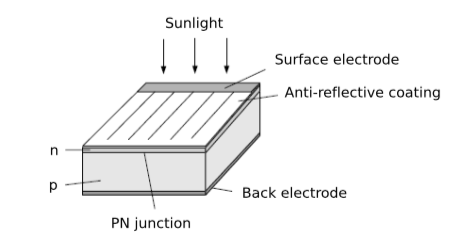
\includegraphics[width=0.6\textwidth]{Fig1} 
    \caption{Structure of a crystalline silicon solar cell.\cite{labmanual}} 
\end{figure}

\subsection{\textsc{Photovoltaic Effect}}
Photovoltaic Effect refers to when the light enters the p-n junction near the solar cell surface, and the energy of the incident photons is larger than the forbidden bandwidth, the incident photons will be absorbed, and the electron-hole pairs will be excited. As a result, the positive charges will accumulate in the p-type area, and the negative ones will accumulated in the n-type one. As a result, a photoelectric potential is generated.
\par The phenomenon we describe above is called the Photovoltaic Effect.

\subsection{\textsc{Solar Cell Parameters}}
Solar cells will generate an electric current $I_{ph}$ from n-type to p-type areas due to the Photovoltaic Effect. Moreover, the device will provide a forward diode current $I_D$ , pointing from p-type to n-type areas. Hence the overall current should be written as:
\begin{equation}
I=I_{\mathrm{ph}}-I_{\mathrm{D}}=I_{\mathrm{ph}}-I_{0}\left[\exp \left(\frac{q V_{\mathrm{D}}}{n k_{\mathrm{B}} T}\right)-1\right]
\end{equation}
where $V_D$ is the junction voltage, $k_B$ refers to the Boltzmann’s constant, n is a theoretical coefficient, which ranges from 1 to 2, q is the electron’s charge, $I_0$ is the diode inverse saturation current, and T is the temperature.
\par Furthermore, if we ignore internal resistance $R_s$, Eq.(1) can be rewritten as:
\begin{equation}
I=I_{\mathrm{ph}}-I_{0}\left[\exp \left(\frac{q V}{n k_{\mathrm{B}} T}\right)-1\right]
\end{equation}
According to Eq.(2), we have:
\begin{itemize}
\item[1.] If the circuit is short circuit, (In other words, V = 0), the short-circuit current is 
		\begin{center}
		$ I_{SC} = I_{ph} $
		\end{center}
\item[2.] On the other hand, if the circuit is open circuit, (In other words, I = 0), the open-circuit voltage is 
		\begin{center}
		$\displaystyle V_{\mathrm{oc}}=\frac{n k_{\mathrm{B}} T}{q} \ln \left(\frac{I_{\mathrm{sc}}}{I_{0}}+1\right) $
		\end{center}
\end{itemize}

If there exist a load resistance R, the I-V relation curve could be determined by changing the resistance. As shown in Fig.2. $R_m$ is the resistance where the output power reaches its maximum value $P_m$, which can be written as:
\begin{center}
$P_m = I_m V_m$
\end{center}
where $I_m$ and $V_m$ are the current and voltage when the output power is maximum and thus they are called optimal operating current and optimal operating voltage respectively.
\par Hence, we can determine the fill factor through Eq.(3) now:
\begin{equation}
F F=\frac{P_{\mathrm{m}}}{V_{\mathrm{oc}} I_{\mathrm{sc}}}=\frac{V_{\mathrm{m}} I_{\mathrm{m}}}{V_{\mathrm{oc}} I_{\mathrm{sc}}}
\end{equation}
Note that the fill factor is importance because it measure the output power. In other words, the greater the fill factor is, the greater the output power is. Also, fill factor is influenced by a variety of factors, including incident light intensity, the theoretical coefficient n, the forbidden bandwidth, and the resistance, etc.
\par Another important parameter is conversion efficiency $\eta$, which can be expressed as:
\begin{equation}
\eta=\frac{P_{\mathrm{m}}}{P_{\mathrm{in}}} \times 100 \%
\end{equation}
where $P_{in}$ refers to the total power incident on the cell.

\begin{figure}[htb] 
    \centering
    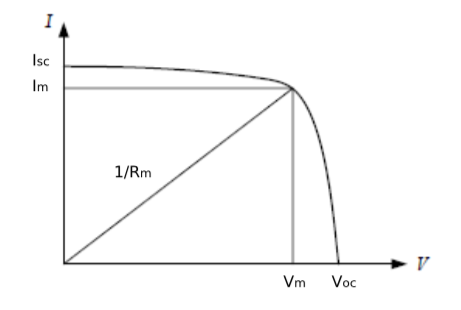
\includegraphics[width=0.55\textwidth]{Fig2} 
    \caption{The current-voltage characteristics of a solar cell.\cite{labmanual}} 
\end{figure}

\subsection{\textsc{Solar Cell Equivalent Circuit}}
A solar cell could be considered being composed of a p-n junction diode D and a constant current source $I_{ph}$, together with a series resistance $R_s$ and a parallel resistance $R_{sh}$. The equivalent circuit is shown in Fig.3, and we can find the following relationships:
\begin{equation}
I=I_{\mathrm{ph}}-I_{0}\left\{\exp \left[\frac{q\left(V+R_{\mathrm{s}} I\right)}{n k_{\mathrm{B}} T}\right]-1\right\}-\frac{V+R_{\mathrm{s}} I}{R_{\mathrm{sh}}}
\end{equation}
When we increase $R_{sh}$ and decrease $R_s$, we will have a higher output power.

\begin{figure}[htb] 
    \centering
    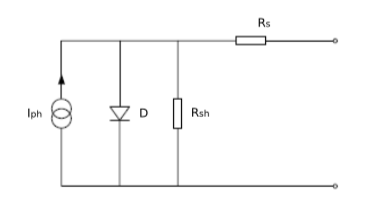
\includegraphics[width=0.5\textwidth]{Fig3} 
    \caption{Solar cell equivalent circuit.\cite{labmanual}} 
\end{figure}

%----------------------------------------------------------------------------------------
%	SECTION 3
%----------------------------------------------------------------------------------------
\section{\textsc{Apparatus and Experimental Setup}}
In this lab, we will use the following apparatuses:
\begin{itemize}
\item A 300W tungsten-halogen lamp serving as a radiation source
\item A photovoltaic device (5 W)
\item Two digital multimeters
\item Two adjustable resistors
\item A solar power meter
\item A measuring tape
\item A wiring board
\end{itemize}


\begin{table}[H]
\begin{center}
\begin{tabular}{|c|c|}
\hline
Quantity & Precision \\ \hline
DC voltage & $\pm(0.5\% + 0.01)$ {[}V{]} \\ \hline
DC current & $\pm(1.5\% + 0.1)$ {[}mA{]} \\ \hline
distance & $\pm 0.1 $ {[}cm{]} \\ \hline
solar power & $\pm 10$ {[}$W/m^2${]} \\ \hline
\end{tabular}
\caption{Multimeter precision.}
\end{center}
\end{table}


%----------------------------------------------------------------------------------------
%	SECTION 4
%----------------------------------------------------------------------------------------
\section{\textsc{Procedures \cite{labmanual}}}
\begin{itemize}
\item[1.] First, we turn on both the light and the fan. Then we wait for at least five minutes, in order to let the light reach its working intensity.
\item[2.] Second, we design a measuring circuit with the photovoltaic device, multimeters set in an appropriate range, and the resistance. Connect the elements into a circuit using the provided wiring board.
\item[3.] Third, we Work in pairs. Adjust the distance between the light source and the photovoltaic device until the $V_{oc}$ and $I_{sc}$ of the two devices are about the same. Measure the solar power by the provided solar power meter. By changing the resistance and measuring the relevant current and voltage, we can plot the I-V characteristics. Note that the plot should be in the following conditions:
\begin{itemize}
\item Two devices in series
\item Two devices in parallel
\item A single device with difference distance
\end{itemize}
\item[4.] Fourth, we change the distance between the light source and the photovoltaic device and measure the I–V characteristics curves and the values of $V_{oc}$ and $I_{sc}$ in a single-device configuration. The new distance should be about 80\% or 120\% of the original one. Measure the solar power at this distance.
\item[5.] Finally, with the help of the computer, we plot the following curve:
\begin{itemize}
\item The I–V characteristics curve
\item Determine the values of $I_{sc}$, $V_{oc}$, $P_m$, $I_m$, $V_m$, $R_m$, $F F$ , and $\eta$ by plotting the graph of the output power vs. the voltage.
\end{itemize}
\end{itemize}



%----------------------------------------------------------------------------------------
%	SECTION 5
%----------------------------------------------------------------------------------------
\section{\textsc{Results}}
\subsection{\textsc{Measurement data for Area and Solar power}}
\begin{table}[H]
\begin{center}
\begin{tabular}{|c|c|c|c|}
\hline
length {[}cm{]} & $u_{length}$ {[}cm{]} & width {[}cm{]} & $u_{width}$ {[}cm{]} \\ \hline
26.1 & 0.1 & 20.9 & 0.1 \\ \hline
\end{tabular}
\caption{Measurement data for area.}
\end{center}
\end{table}

The measurement data for length and width are recorded in Table 2. Hence, the area can be calculated as follows (Detailed calculations for uncertainties are shown in A.1):
\begin{center}
$ \displaystyle S = length \times width = 545 \pm 3[cm^2] $
\end{center}
with a relative error $r_{S} = 0.6\%$.


\begin{table}[H]
\begin{center}
\begin{tabular}{|c|c|c|c|c|c|c|c|c|}
\hline
 & 1 & 2 & 3 & 4 & 5 & 6 & average & $u_{average}$ \\ \hline
$P_{80.6}$ $[W/m^2]$ $\pm$ 10 $[W/m^2]$ & 265 & 273 & 255 & 263 & 285 & 287 & 271 & 20 \\ \hline
$P_{101.5}$ $[W/m^2]$ $\pm$ 10 $[W/m^2]$ & 234 & 220 & 162 & 172 & 184 & 190 & 194 & 30 \\ \hline
\end{tabular}
\caption{Measurement data for solar power.}
\end{center}
\end{table}
For measurements for solar power, the data are recorded in Table 3. Hence, the average solar power for the distance $x = 80.6 cm$ can be calculated as follows (Detailed calculations for uncertainties are shown in A.2.1):
\begin{center}
$ \displaystyle \overline{P_{80.6}} = \frac{\sum_{i=1}^6P_i}{6} = \frac{265 + 273 + 255 + 263 + 285 + 287}{6} = 271 \pm 20 [W/m^2] $
\end{center}
with a relative error $r_{P,80.6} = 7\%$
\par For $x = 101.5 cm$, the process is similar, and we obtain (Detailed calculations for uncertainties are shown in A.2.2):
\begin{center}
$ \displaystyle \overline{P_{101.5}} = \frac{\sum_{i=1}^6P_i}{6} = \frac{234 + 220 + 162 + 172 + 184 + 190}{6} = 194 \pm 30 [W/m^2] $
\end{center}
with a relative error $r_{P,101.5} = 15\%$
\par Now, based on the area $S$ we have calculated before, we can calculate the value of $P_{in}$ as follows (Detailed calculations for uncertainties are shown in A.2.3):
\begin{center}
$P_{in,80.6} = S \times P_{80.6} = 0.0545 \times 271 =  14.8 \pm 1.1 [W] $
\end{center}
with a relative error $r_{P_{in,80.6}} = 7\%$.
\par Similarly, when the distance is 101.5 cm, we have:
\begin{center}
$P_{in,101.5} = S \times P_{101.5} = 0.0545 \times 194 =  10.6 \pm 1.6 [W] $
\end{center}
with a relative error $r_{P_{in,101.5}} = 15\%$.


\subsection{\textsc{Measurement data for $U_{OC}$ and $I_{SC}$}}

\begin{table}[H]
\begin{center}
\begin{tabular}{|c|c|c|c|c|}
\hline
 & single device at 80.6 cm & single device at 101.5 cm & series & parallel \\ \hline
$U_{OC}$ {[}V{]} & 8.46 & 7.59 & 17.51 & 8.72 \\ \hline
$u_U$ {[}V{]} & 0.05 & 0.05 & 0.10 & 0.05 \\ \hline
$I_{SC}$ {[}mA{]} & 67.6 & 47.0 & 59.2 & 121.2 \\ \hline
$u_I$ {[}mA{]} & 1.1 & 0.8 & 1.0 & 1.9 \\ \hline
\end{tabular}
\caption{Measurement data for $U_{OC}$ and $I_{SC}$.}
\end{center}
\end{table}
In this section, we find out the open circuit voltage and short circuit current. The data are shown in Table 4, and the values with their uncertainties are shown below (Detailed calculations for uncertainties are shown in A.3):
\begin{itemize}
\item[1.] For single device at 80.6 cm,
			\begin{itemize}
			\item[a)] The open circuit voltage $U_{OC} = 8.46 \pm 0.05 [V]$, with a relative error 0.6\%.
			\item[b)] The short circuit current $I_{SC} = 67.6 \pm 1.1 [mA]$, with a relative error 1.6\%.
			\end{itemize}
\item[2.] For single device at 101.5 cm,
			\begin{itemize}
			\item[a)] The open circuit voltage $U_{OC} = 7.59 \pm 0.05 [V]$, with a relative error 0.7\%.
			\item[b)] The short circuit current $I_{SC} = 47.0 \pm 0.8 [mA]$, with a relative error 1.7\%.
			\end{itemize}
\item[3.] For two devices connected in series,
			\begin{itemize}
			\item[a)] The open circuit voltage $U_{OC} = 17.51 \pm 0.10 [V]$, with a relative error 0.6\%.
			\item[b)] The short circuit current $I_{SC} = 59.2 \pm 1.0 [mA]$, with a relative error 1.7\%.
			\end{itemize}
\item[4.] For single device at 80.6 cm, the uncertainties can be calculated as:
			\begin{itemize}
			\item[a)] The open circuit voltage $U_{OC} = 8.72 \pm 0.05 [V]$, with a relative error 0.6\%.
			\item[b)] The short circuit current $I_{SC} = 121.2 \pm 1.9 [mA]$, with a relative error 1.6\%.
			\end{itemize}
\end{itemize}


\subsection{\textsc{Measurement data for U vs. I relation}}
\newpage
\subsubsection{\textsc{Two devices are connected in series}}
In this part, we record the value of $U$ and $I$ when two devices are connected in series. Based on these two data, we can calculate the output power $P$ and the corresponding resistance $R$. Take the second data as a sample calculation, we have $U = 3.90 [V]$ and $I = 53.5 [mA]$. Hence, we obtain:
\begin{center}
$ P = UI = 3.90 \times 53.5 = 209 \pm 4 [mW] $
\end{center}
with a relative error $r_P = 1.9\%$.
\par On the other side, for the resistance, we have:
\begin{center}
$ \displaystyle R = \frac{U}{I} = \frac{3.90}{0.0535} = 72.9 \pm 1.3 [\Omega] $
\end{center}
with a relative error $r_R = 1.8\%$.

\begin{table}[H]
\begin{center}
\begin{tabular}{|c|c|c|c|c|c|c|c|c|}
\hline
\multicolumn{9}{|c|}{In series} \\ \hline
 & U {[}V{]} & $u_U$ {[}V{]} & I {[}mA{]} & $u_I$ {[}mA{]} & P {[}mW{]} & $u_P$ {[}mW{]} & R {[}$\Omega${]} & $u_R$ {[}$\Omega${]} \\ \hline
1 & 0.68 & 0.013 & 58.3 & 1.0 & 39.6 & 1.0 & 11.7 & 0.3 \\ \hline
2 & 3.90 & 0.03 & 53.5 & 0.9 & 209 & 4 & 72.9 & 1.3 \\ \hline
3 & 6.48 & 0.04 & 49.7 & 0.8 & 322 & 6 & 130 & 2 \\ \hline
4 & 7.76 & 0.05 & 47.9 & 0.8 & 372 & 7 & 162 & 3 \\ \hline
5 & 7.97 & 0.05 & 47.6 & 0.8 & 379 & 7 & 167 & 3 \\ \hline
6 & 8.37 & 0.05 & 46.8 & 0.8 & 392 & 7 & 179 & 3 \\ \hline
7 & 8.64 & 0.05 & 46.3 & 0.8 & 400 & 7 & 187 & 3 \\ \hline
8 & 8.80 & 0.05 & 46.1 & 0.8 & 406 & 7 & 191 & 3 \\ \hline
9 & 9.04 & 0.06 & 45.4 & 0.8 & 410 & 7 & 199 & 4 \\ \hline
10 & 9.20 & 0.06 & 45.0 & 0.8 & 414 & 8 & 204 & 4 \\ \hline
11 & 9.33 & 0.06 & 44.7 & 0.8 & 417 & 8 & 209 & 4 \\ \hline
12 & 9.48 & 0.06 & 44.2 & 0.8 & 419 & 8 & 214 & 4 \\ \hline
13 & 9.57 & 0.06 & 44.1 & 0.8 & 422 & 8 & 217 & 4 \\ \hline
14 & 9.75 & 0.06 & 43.8 & 0.8 & 427 & 8 & 223 & 4 \\ \hline
15 & 9.83 & 0.06 & 43.6 & 0.8 & 429 & 8 & 225 & 4 \\ \hline
16 & 9.99 & 0.06 & 43.0 & 0.7 & 430 & 8 & 232 & 4 \\ \hline
17 & 10.10 & 0.06 & 42.8 & 0.7 & 432 & 8 & 236 & 4 \\ \hline
18 & 10.18 & 0.06 & 42.7 & 0.7 & 435 & 8 & 238 & 4 \\ \hline
19 & 10.30 & 0.06 & 42.3 & 0.7 & 436 & 8 & 243 & 4 \\ \hline
20 & 10.52 & 0.06 & 41.8 & 0.7 & 440 & 8 & 252 & 5 \\ \hline
21 & 10.94 & 0.06 & 40.6 & 0.7 & 444 & 8 & 269 & 5 \\ \hline
22 & 11.32 & 0.07 & 39.6 & 0.7 & 448 & 8 & 286 & 5 \\ \hline
23 & 12.44 & 0.07 & 36.5 & 0.6 & 454 & 8 & 341 & 6 \\ \hline
24 & 14.16 & 0.08 & 29.3 & 0.5 & 415 & 8 & 483 & 9 \\ \hline
25 & 16.03 & 0.09 & 16.3 & 0.3 & 261 & 6 & 983 & 20 \\ \hline
\end{tabular}
\caption{Measurement data for $U$ vs. $I$ relation (in series).}
\end{center}
\end{table}


\subsubsection{\textsc{Two devices are connected in parallel}}
In this part, we record the value of $U$ and $I$ when two devices are connected in parallel. Based on these two data, we can calculate the output power $P$ and the corresponding resistance $R$. Take the second data as a sample calculation, we have $U = 2.04 [V]$ and $I = 114.5 [mA]$. Hence, we obtain:
\begin{center}
$ P = UI = 2.04 \times 114.5 = 234 \pm 4 [mW] $
\end{center}
with a relative error $r_P = 1.7\%$.
\par On the other side, for the resistance, we have:
\begin{center}
$ \displaystyle R = \frac{U}{I} = \frac{2.04}{0.1145} = 17.8 \pm 0.3 [\Omega] $
\end{center}
with a relative error $r_R = 1.7\%$.

\begin{table}[H]
\begin{center}
\begin{tabular}{|c|c|c|c|c|c|c|c|c|}
\hline
\multicolumn{9}{|c|}{In parallel} \\ \hline
 & U {[}V{]} & $u_U$ {[}V{]} & I {[}mA{]} & $u_I$ {[}mA{]} & P {[}mW{]} & $u_P$ {[}mW{]} & R {[}$\Omega${]} & $u_R$ {[}$\Omega${]} \\ \hline
    1     & 0.83  & 0.014  & 120.6  & 1.9   & 100  & 2   & 6.9   & 0.2  \\ \hline
    2     & 2.04  & 0.02  & 114.5  & 1.8   & 234   & 4     & 17.8  & 0.3  \\ \hline
    3     & 3.16  & 0.03  & 107.7  & 1.7   & 340   & 6     & 29.3  & 0.5  \\ \hline
    4     & 3.92  & 0.03  & 101.2  & 1.6   & 397   & 7     & 38.7  & 0.7  \\ \hline
    5     & 4.22  & 0.03  & 98.4  & 1.6   & 415   & 7     & 42.9  & 0.8  \\ \hline
    6     & 4.55  & 0.03  & 95.5  & 1.5   & 435   & 8     & 47.6  & 0.8  \\ \hline
    7     & 4.99  & 0.03  & 91.1  & 1.5   & 455   & 8     & 54.8  & 1.0  \\ \hline
    8     & 5.14  & 0.04  & 89.1  & 1.4   & 458   & 8     & 57.7  & 1.0  \\ \hline
    9     & 5.33  & 0.04  & 87.1  & 1.4   & 464   & 8     & 61.2  & 1.1  \\ \hline
    10    & 5.51  & 0.04  & 85.1  & 1.4   & 469   & 8     & 64.7  & 1.1  \\ \hline
    11    & 5.69  & 0.04  & 82.9  & 1.3   & 472   & 8     & 68.6  & 1.2  \\ \hline
    12    & 5.85  & 0.04  & 80.8  & 1.3   & 473   & 8     & 72.4  & 1.3  \\ \hline
    13    & 5.99  & 0.04  & 78.9  & 1.3   & 473   & 8     & 75.9  & 1.3  \\ \hline
    14    & 6.07  & 0.04  & 77.9  & 1.3   & 473   & 8     & 77.9  & 1.4  \\ \hline
    15    & 6.16  & 0.04  & 76.2  & 1.2   & 469   & 8     & 80.8  & 1.4  \\ \hline
    16    & 6.32  & 0.04  & 73.8  & 1.2   & 466   & 8     & 85.6  & 1.5  \\ \hline
    17    & 6.52  & 0.04  & 71.0  & 1.2   & 463   & 8     & 91.8  & 1.6  \\ \hline
    18    & 6.75  & 0.04  & 67.1  & 1.1   & 453   & 8     & 100.6  & 1.8  \\ \hline
    19    & 6.96  & 0.04  & 62.4  & 1.0   & 434   & 8     & 112   & 2  \\ \hline
    20    & 7.31  & 0.05  & 54.2  & 0.9   & 396   & 7     & 135   & 2  \\ \hline
    21    & 7.56  & 0.05  & 47.5  & 0.8   & 359   & 7     & 159   & 3  \\ \hline
    22    & 7.78  & 0.05  & 40.7  & 0.7   & 317   & 6     & 191   & 4  \\ \hline
    23    & 7.98  & 0.05  & 33.7  & 0.6   & 269   & 5     & 237   & 5  \\ \hline
    24    & 8.36  & 0.05  & 17.4  & 0.4   & 145   & 3     & 480   & 10  \\ \hline
    25    & 8.52  & 0.05  & 9.2   & 0.2   & 78    & 2     & 926   & 30  \\ \hline
\end{tabular}
\caption{Measurement data for $U$ vs. $I$ relation (in parallel).}
\end{center}
\end{table}


\subsubsection{\textsc{Single device at the distance 80.6 cm}}
In this part, we record the value of $U$ and $I$ when a single devices is placed at 80.6 cm. Based on these two data, we can calculate the output power $P$ and the corresponding resistance $R$. Take the second data as a sample calculation, we have $U = 1.01 [V]$ and $I = 65.8 [mA]$. Hence, we obtain:
\begin{center}
$ P = UI = 1.01 \times 65.8 = 66.5 \pm 1.5 [mW] $
\end{center}
with a relative error $r_P = 2\%$.
\par On the other side, for the resistance, we have:
\begin{center}
$ \displaystyle R = \frac{U}{I} = \frac{1.01}{0.0658} = 15.3 \pm 0.3 [\Omega] $
\end{center}
with a relative error $r_R = 2\%$.

\begin{table}[H]
\begin{center}
\begin{tabular}{|c|c|c|c|c|c|c|c|c|}
\hline
\multicolumn{9}{|c|}{Single device at 80.6 cm} \\ \hline
 & U {[}V{]} & $u_U$ {[}V{]} & I {[}mA{]} & $u_I$ {[}mA{]} & P {[}mW{]} & $u_P$ {[}mW{]} & R {[}$\Omega${]} & $u_R$ {[}$\Omega${]} \\ \hline
 1     & 0.46  & 0.012  & 67.0  & 1.1   & 30.8  & 1.0   & 6.9   & 0.2  \\ \hline
    2     & 1.01  & 0.02  & 65.8  & 1.1   & 66.5  & 1.5   & 15.3  & 0.3  \\ \hline
    3     & 1.49  & 0.02  & 64.3  & 1.1   & 95.8  & 1.9   & 23.2  & 0.5  \\ \hline
    4     & 2.20  & 0.02  & 60.7  & 1.0   & 134   & 3     & 36.2  & 0.7  \\ \hline
    5     & 2.95  & 0.02  & 57.6  & 1.0   & 170   & 3     & 51.2  & 1.0  \\ \hline
    6     & 3.49  & 0.03  & 54.9  & 0.9   & 192   & 4     & 63.6  & 1.2  \\ \hline
    7     & 3.98  & 0.03  & 52.1  & 0.9   & 207   & 4     & 76.4  & 1.4  \\ \hline
    8     & 4.52  & 0.03  & 48.4  & 0.8   & 219   & 4     & 93.4  & 1.7  \\ \hline
    9     & 4.94  & 0.03  & 45.4  & 0.8   & 224   & 4     & 109   & 2  \\ \hline
    10    & 5.12  & 0.04  & 44.1  & 0.8   & 226   & 4     & 116   & 2  \\ \hline
    11    & 5.20  & 0.04  & 43.4  & 0.8   & 226   & 4     & 120   & 2  \\ \hline
    12    & 5.34  & 0.04  & 42.4  & 0.7   & 226   & 4     & 126   & 2  \\ \hline
    13    & 5.44  & 0.04  & 41.6  & 0.7   & 226   & 4     & 131   & 2  \\ \hline
    14    & 5.58  & 0.04  & 40.5  & 0.7   & 226   & 4     & 138   & 3  \\ \hline
    15    & 5.71  & 0.04  & 39.5  & 0.7   & 226   & 4     & 145   & 3  \\ \hline
    16    & 5.89  & 0.04  & 38.1  & 0.7   & 224   & 4     & 155   & 3  \\ \hline
    17    & 6.01  & 0.04  & 37.2  & 0.7   & 224   & 4     & 162   & 3  \\ \hline
    18    & 6.14  & 0.04  & 36.2  & 0.6   & 222   & 4     & 170   & 3  \\ \hline
    19    & 6.34  & 0.04  & 34.5  & 0.6   & 219   & 4     & 184   & 4  \\ \hline
    20    & 6.54  & 0.04  & 32.4  & 0.6   & 212   & 4     & 202   & 4  \\ \hline
    21    & 6.85  & 0.04  & 28.8  & 0.5   & 197   & 4     & 238   & 5  \\ \hline
    22    & 7.18  & 0.05  & 24.3  & 0.5   & 174   & 4     & 295   & 6  \\ \hline
    23    & 7.53  & 0.05  & 18.5  & 0.4   & 139   & 3     & 407   & 9  \\ \hline
    24    & 7.80  & 0.05  & 13.5  & 0.3   & 105   & 2     & 578   & 10  \\ \hline
    25    & 8.15  & 0.05  & 7.2   & 0.2   & 58.7  & 1.7   & 1132  & 30  \\ \hline
\end{tabular}
\caption{Measurement data for $U$ vs. $I$ relation (at 80.6 cm).}
\end{center}
\end{table}


\subsubsection{\textsc{Single device at the distance 101.5 cm}}
In this part, we record the value of $U$ and $I$ when a single devices is placed at 101.5 cm. Based on these two data, we can calculate the output power $P$ and the corresponding resistance $R$. Take the second data as a sample calculation, we have $U = 1.36 [V]$ and $I = 43.5 [mA]$. Hence, we obtain:
\begin{center}
$ P = UI = 1.36 \times 43.5 = 59.2 \pm 1.3 [mW] $
\end{center}
with a relative error $r_P = 2\%$.
\par On the other side, for the resistance, we have:
\begin{center}
$ \displaystyle R = \frac{U}{I} = \frac{1.36}{0.0435} = 31.3 \pm 0.7 [\Omega] $
\end{center}
with a relative error $r_R = 2\%$.

\begin{table}[H]
\begin{center}
\begin{tabular}{|c|c|c|c|c|c|c|c|c|}
\hline
\multicolumn{9}{|c|}{Single device at 101.5 cm} \\ \hline
 & U {[}V{]} & $u_U$ {[}V{]} & I {[}mA{]} & $u_I$ {[}mA{]} & P {[}mW{]} & $u_P$ {[}mW{]} & R {[}$\Omega${]} & $u_R$ {[}$\Omega${]} \\ \hline
 1     & 0.32  & 0.012  & 46.8  & 0.8   & 15.0  & 0.6   & 6.8   & 0.3  \\ \hline
    2     & 1.36  & 0.02  & 43.5  & 0.8   & 59.2  & 1.3   & 31.3  & 0.7  \\ \hline
    3     & 2.15  & 0.02  & 41.0  & 0.7   & 88.2  & 1.8   & 52.4  & 1.0  \\ \hline
    4     & 2.66  & 0.02  & 39.3  & 0.7   & 105   & 2     & 67.7  & 1.3  \\ \hline
    5     & 3.04  & 0.03  & 37.8  & 0.7   & 115   & 2     & 80.4  & 1.6  \\ \hline
    6     & 3.47  & 0.03  & 35.7  & 0.6   & 124   & 2     & 97.2  & 1.9  \\ \hline
    7     & 3.84  & 0.03  & 33.8  & 0.6   & 130   & 3     & 114   & 2  \\ \hline
    8     & 4.16  & 0.03  & 31.9  & 0.6   & 133   & 3     & 130   & 3  \\ \hline
    9     & 4.21  & 0.03  & 31.7  & 0.6   & 133   & 3     & 133   & 3  \\ \hline
    10    & 4.35  & 0.03  & 30.9  & 0.6   & 134   & 3     & 141   & 3  \\ \hline
    11    & 4.47  & 0.03  & 30.3  & 0.6   & 135   & 3     & 148   & 3  \\ \hline
    12    & 4.59  & 0.03  & 29.5  & 0.5   & 135   & 3     & 156   & 3  \\ \hline
    13    & 4.71  & 0.03  & 28.7  & 0.5   & 135   & 3     & 164   & 3  \\ \hline
    14    & 4.81  & 0.03  & 28.0  & 0.5   & 135   & 3     & 172   & 3  \\ \hline
    15    & 4.91  & 0.03  & 27.5  & 0.5   & 135   & 3     & 179   & 4  \\ \hline
    16    & 5.05  & 0.04  & 26.5  & 0.5   & 134   & 3     & 191   & 4  \\ \hline
    17    & 5.21  & 0.04  & 25.6  & 0.5   & 133   & 3     & 204   & 4  \\ \hline
    18    & 5.34  & 0.04  & 24.8  & 0.5   & 132   & 3     & 215   & 4  \\ \hline
    19    & 5.57  & 0.04  & 23.2  & 0.4   & 129   & 3     & 240   & 5  \\ \hline
    20    & 5.78  & 0.04  & 21.6  & 0.4   & 125   & 3     & 268   & 6  \\ \hline
    21    & 5.96  & 0.04  & 20.1  & 0.4   & 120   & 3     & 297   & 6  \\ \hline
    22    & 6.20  & 0.04  & 18.0  & 0.4   & 112   & 2     & 344   & 7  \\ \hline
    23    & 6.43  & 0.04  & 15.6  & 0.3   & 100   & 2     & 412   & 9  \\ \hline
    24    & 6.81  & 0.04  & 11.3  & 0.3   & 77.0  & 1.9   & 603   & 20  \\ \hline
    25    & 7.10  & 0.05  & 6.1   & 0.2   & 43.3  & 1.4   & 1164  & 40  \\ \hline
\end{tabular}
\caption{Measurement data for $U$ vs. $I$ relation (at 101.5 cm).}
\end{center}
\end{table}

\subsubsection{\textsc{Graph for I-V characteristics}}
Based on our data in Table 5, 6, 7, and 8, we are able to use \textit{Origin} to plot the graph of I-V characteristics. The result is shown in Fig.(\ref{IU}).
\begin{figure}[htb] 
    \centering
    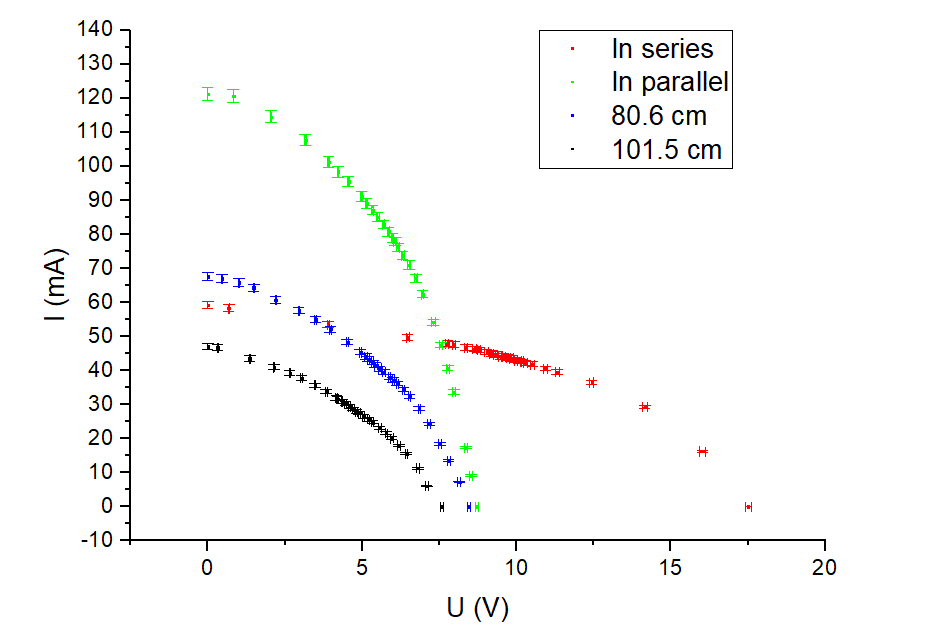
\includegraphics[width=0.9\textwidth]{IU} 
    \caption{The I-V relation in different case.} 
    \label{IU}    
\end{figure}

From Fig.(\ref{IU}), we find that with the \textbf{increase} of the voltage $V$, the current $I$ \textbf{decrease}. Besides, when the distance between the light source and the solar device become \textbf{smaller}, the corresponding $V$ and $I$ become \textbf{higher}. Eventually, if the solar cell devices are connected in series, the voltage will be \textbf{higher}, with approximately \textbf{twice} the original value, and if they are connected in parallel, the current will be \textbf{higher}, also with approximately \textbf{twice} the original value.
\par In the figure, the Open-circuit voltage is included, with the corresponding Open-Circuit Current and its uncertainty has the value zero. Also, for the Short-circuit current, the corresponding Short-circuit voltage and its uncertainty has the value zero. Details about the errors will be discussed later.

\subsubsection{\textsc{Graph for P-V characteristics}}
Based on our data in Table 5, 6, 7, and 8, we are able to use \textit{Origin} to plot the graph of P-V characteristics. The result is shown in Fig.(\ref{PU}).

\par From Fig.(\ref{PU}), we find that with the \textbf{increase} of the voltage $V$, the power $P$ first \textbf{increase} then \textbf{decrease}, and thus has a maximum value. Besides, when the distance between the light source and the solar device become \textbf{smaller}, the corresponding $P$ and $V$ become \textbf{higher}. Eventually, if the solar cell devices are connected in series, the voltage will be \textbf{higher}, with approximately \textbf{twice} the original value. However, the maximum power are roughly the \textbf{same} regardless of series and parallel connection. Details about the errors will be discussed later.

\begin{figure}[H] 
    \centering
    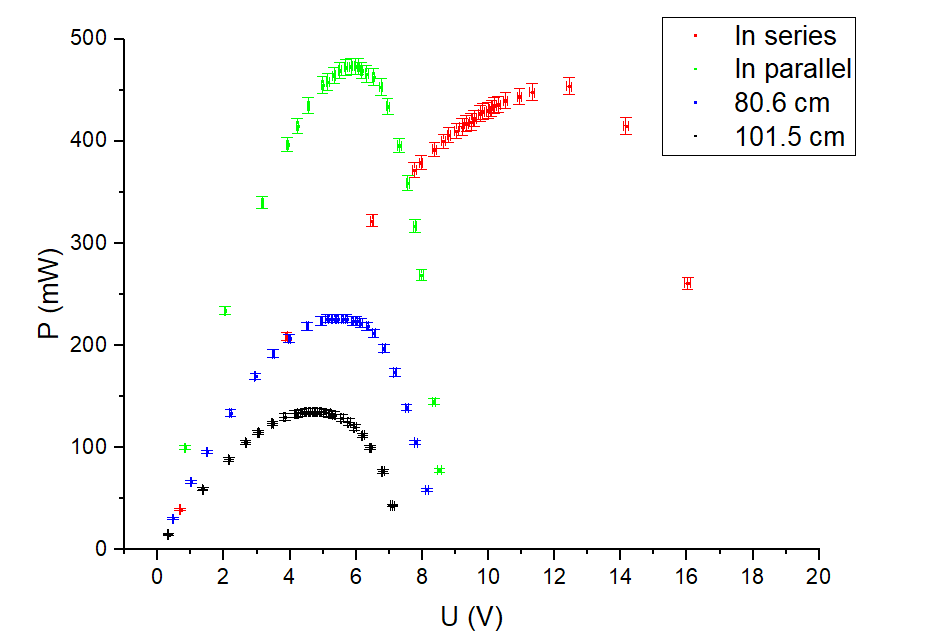
\includegraphics[width=0.9\textwidth]{PU} 
    \caption{The P-V relation in different case.} 
    \label{PU}    
\end{figure}

\subsubsection{\textsc{Graph for P-R characteristics}}

\begin{figure}[H] 
    \centering
    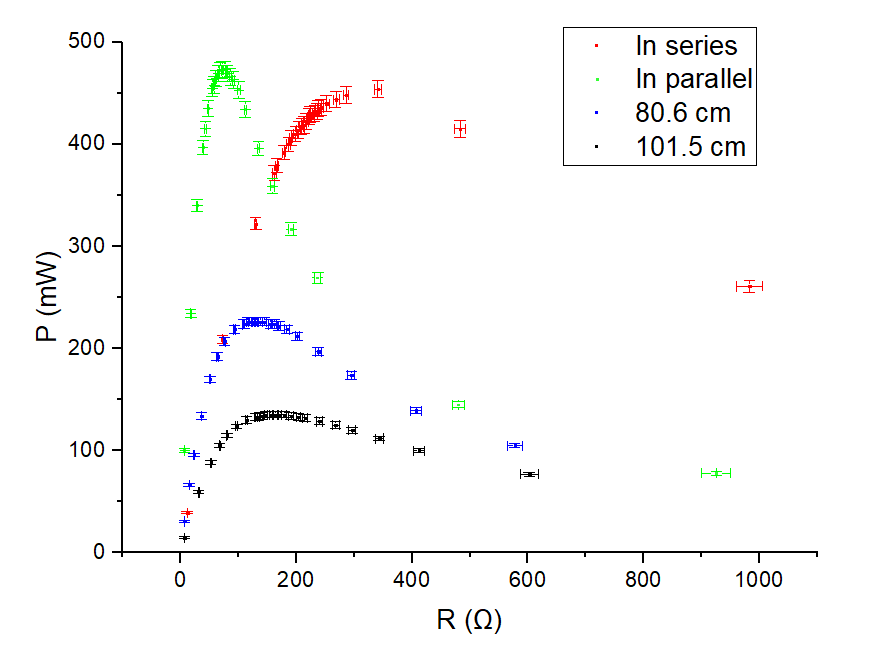
\includegraphics[width=0.9\textwidth]{PR} 
    \caption{The P-R relation in different case.} 
    \label{PR}    
\end{figure}

Based on our data in Table 5, 6, 7, and 8, we are able to use \textit{Origin} to plot the graph of P-R characteristics. The result is shown in Fig.(\ref{PR}).

\par From Fig.(\ref{PR}), we find that with the \textbf{increase} of the resistance $R$, the power $P$ first \textbf{increase} then \textbf{decrease}, and thus has a maximum value. Besides, when the distance between the light source and the solar device become \textbf{smaller}, the corresponding $P$ become \textbf{higher}. Eventually, if the solar cell devices are connected in series or in parallel, the maximum power is \textbf{larger}, with roughly \textbf{twice} the value of a single device. Details about the errors will be discussed later.

\subsection{\textsc{Fill Factor and Conversion Efficiency}}
In this section, we find out the fill factor and conversion efficiency based on the data and calculations above. First, for the fill factor, we have (Detailed calculation for uncertainties will be shown in A.5)
\begin{center}
$\displaystyle FF = \frac{P_m}{V_{OC}I_{SC}} $
\end{center}
Hence, we have:
\begin{itemize}
\item[1.] For the two devices connected in series:
			\begin{center}
			$\displaystyle FF_{series} = \frac{P_m}{V_{OC}I_{SC}} = \frac{454}{17.51\times 59.2} = 0.438 \pm 0.011 $
			\end{center}
			with a relative error $r_{FF} = 3 \%$. 
\item[2.] For the two devices connected in parallel:
			\begin{center}
			$\displaystyle FF_{parallel} = \frac{P_m}{V_{OC}I_{SC}} = \frac{473}{8.72\times 121.2} = 0.448 \pm 0.011 $
			\end{center}
			with a relative error $r_{FF} = 2 \%$. 
\item[3.] For a single device with a distance 80.6 cm:
			\begin{center}
			$\displaystyle FF_{80.6} = \frac{P_m}{V_{OC}I_{SC}} = \frac{226}{8.46\times 67.6} = 0.395 \pm 0.010 $
			\end{center}
			with a relative error $r_{FF} = 3 \%$. 
\item[4.] For a single device with a distance 101.5 cm
			\begin{center}
			$\displaystyle FF_{101.5} = \frac{P_m}{V_{OC}I_{SC}} = \frac{135}{7.59\times 47.0} = 0.378 \pm 0.011 $
			\end{center}
			with a relative error $r_{FF} = 3 \%$. 
\end{itemize}
\par Then, we calculate the conversion efficiency, which is given by:
\begin{center}
$\displaystyle \eta = \frac{P_m}{P_{in}}\times 100\%$
\end{center}
Hence, we have:
\begin{itemize}
\item[1.] For a single device with a distance 80.6 cm:
			\begin{center}
			$\displaystyle \eta = \frac{P_m}{P_{in}}\times 100\% = \frac{0.226}{14.8}\times 100\% = 1.53\% \pm 0.12\% $
			\end{center}
			with a relative error $r_{\eta} = 8\%$.
\item[2.] For a single device with a distance 101.5 cm:
			\begin{center}
			$\displaystyle \eta = \frac{P_m}{P_{in}}\times 100\% = \frac{0.135}{10.6}\times 100\% = 1.27\% \pm 0.19\% $
			\end{center}			
			with a relative error $r_{\eta} = 15\%$.
\end{itemize}

In all, based on the calculations above, we can obtain Table 9, which includes all the information we need.

\begin{table}[H]
\begin{center}
\begin{tabular}{|c|c|c|c|c|c|c|c|c|}
\hline
 & $U_{OC}$ {[}V{]} & $I_{SC}$ {[}mA{]} & $P_m$ {[}mW{]} & $U_m$ {[}V{]} & $I_m$ {[}mA{]} & $R_m$ {[}$\Omega${]} & FF & $\eta$ \\ \hline
80.6 cm & 8.46 & 67.6 & 226 & 5.34 & 42.4 & 126 & 0.395 & 1.53\% \\ \hline
Uncertainty & 0.05 & 1.1 & 4 & 0.04 & 0.7 & 2 & 0.010 & 0.12\% \\ \hline
101.5 cm & 7.59 & 47.0 & 135 & 4.71 & 28.7 & 164 & 0.378 & 1.27\% \\ \hline
Uncertainty & 0.05 & 0.8 & 3 & 0.03 & 0.5 & 3 & 0.011 & 0.19\% \\ \hline
In series & 17.51 & 59.2 & 454 & 12.44 & 36.5 & 341 & 0.438 & / \\ \hline
Uncertainty & 0.10 & 1.0 & 8 & 0.07 & 0.6 & 6 & 0.011 & / \\ \hline
In parallel & 8.72 & 121.2 & 473 & 5.99 & 78.9 & 75.9 & 0.448 & / \\ \hline
Uncertainty & 0.05 & 1.9 & 8 & 0.04 & 1.3 & 1.3 & 0.011 & / \\ \hline
\end{tabular}
\caption{Fill Factor and Conversion Efficiency.}
\end{center}
\end{table}

%----------------------------------------------------------------------------------------
%	SECTION 6
%----------------------------------------------------------------------------------------

\section{\textsc{Conclusion and Discussion}}
\subsection{\textsc{Discussion}}
In this lab, generally speaking we have done a satisfactory job. However, some errors still occur. Now we make some analysis on the errors in this lab and their possible improvements.
\begin{itemize}
\item[1.] For the measurement for the area, our result is quite accurate. Hence we only measure the quantity once and obtain a small uncertainty.
\item[2.] For the measurement of solar power, we measured for six times. However, we can observe that these data vary a lot, with a largest deviation 72$[W/m^2]$. This result in a large type-A uncertainty, and finally contribute to the large overall uncertainty. The possible reasons may be:
		\begin{itemize}
		\item[(a)] The lamp doesn't shine on the solar cell horizontally. Instead, there is a small inclination leading to the large deviation of solar power on different corner.
		\item[(b)] The solar meter doesn't face directly to the lamp. Instead, there exist some inclination.
		\item[(c)] The lamp doesn't shine on the center of the solar cell. As a result, the distribution of solar power will have a large difference.
		\item[(d)] Light from other groups or other heat sources nearby may result in a large difference. 
		\end{itemize}

		[Possible Solutions]:
		\begin{itemize}
		\item[(a)] Do the experiment in a isolated environment without others' interference. Or use board between different groups to prevent the influence from others.
		\item[(b)] Use a scale to make sure that lamp shine on the cell horizontally.
		\item[(c)] Use a meter to make sure that the light shine on the center of the solar cell.
		\end{itemize}

\item[3.] For the measurement of $U_{OC}$ and $I_{SC}$, our relative error are generally less than 2\%. And we can see that our uncertainties only come from type-B uncertainties, which is restricted by our instruments.

		[Possible Solutions]:
		\begin{itemize}
		\item[(a)] We can improve our apparatus to have a better resolution to reduce the type-B uncertainties.
		\item[(b)] For some measurements, we may change the scale of the multimeter to a suitable value. In this way our result will be more accurate.
		\end{itemize}
		
\item[4.] For the measurement of $U$ vs. $I$ characteristics, we use \textit{Origin} to plot some figures and obtain our results. However, some errors still occur, and we find that 
		\begin{itemize}
		\item[(a)] On the graph, we didn't collect enough points when the power reaches maximum in the series connection case. This may lead to misreading for the $P_m$.
		\item[(b)] For some set of data, our maximum value of voltage and current are quite different from the Open-Circuit voltage and Short-Circuit current. This is because the wires or other components have inner resistance in reality, which we ignore theoretically. Moreover, this may because after we measured $V_{OC}$ and $I_{SC}$, it has been a long time, and the light shining on the solar cell may be different, which leads to the errors.
		\end{itemize}

		[Possible Solutions]:
		\begin{itemize}
		\item[(a)] Compared with the 25 sets of data, we can collect more sets of data. For instance, we can collect 50 sets of data so that our graph will be more completed.
		\item[(b)] Before we start measuring the result, we can first adjust the apparatus to observe where the maximum power may occur and record the corresponding voltage and current. Then, after we begin our experiment, when approaching the particular value, we slow down and collect more data.
		\item[(c)] We can change the scale of multimeter if it is needed.
		\item[(d)] We can take into consideration the inner resistance of wires and other electronic components.
		\item[(e)] After we begin our experiment, we should not touch our light source or the solar cell to decrease the light changing.
		\item[(f)] We can use better instruments to do our experiments. For instance, we can use better wires with less inner resistance.
		\end{itemize}
				
\item[5.] For the measurement of fill factor and conversion efficiency, we find that though our relative error of the results are low, both the value of fill factor and conversion efficiency are much smaller than expected. Possible reasons may be: 
		\begin{itemize}
		\item[(a)] Because the solar cell is too old and out-of-date, its efficiency decrease.
		\item[(b)] Due to the inner resistance or other reasons, the hated may be consumed in other ways, resulting in the loss of power. 
		\item[(c)] The lamp doesn't face directly to the lamp and causes some energy loss.
		\end{itemize}


		[Possible Solutions]:
		\begin{itemize}
		\item[(a)] We can use a newer solar cell to conduct our experiment.
		\item[(b)] Before measurements, calibrate the light source so that it face horizontally to the solar cell to prevent power loss.
		\end{itemize}
\end{itemize}

\subsection{\textsc{Conclusion}}
During the experiment, we have accomplished our tasks successfully, and we have really learned a lot during the process, including:
\begin{itemize}
\item[1.] We understand the basic working principle of a solar cell.
\item[2.] We learn the I-V, P-V, and P-R characteristics of a power cell. 
\item[3.] We know how to build up a circuit to measure the open circuit voltage and short circuit current for different connection of solar cells.
\end{itemize}
\par To sum up, we find the following conclusion based on our results:
\begin{itemize}
\item[1.] For the I-V characteristics, we find that 
		\begin{itemize}
		\item[(a)] With the increase of the voltage V , the current I decrease.
		\item[(b)] When the distance between the light source and the solar device become smaller, the corresponding V and I become higher. 
		\item[(c)] If the solar cell devices are connected in series, the voltage will be higher, with approximately twice the original value, and if they are connected in parallel, the current will be higher, also with approximately twice the original value.
		\end{itemize}

\item[2.] For the P-V characteristics, we find that 
		\begin{itemize}
		\item[(a)] With the increase of the voltage V , the power P first increase then decrease, and thus has a maximum value. 
		\item[(b)] When the distance between the light source and the solar device become smaller, the corresponding P and V become higher.
		\item[(c)] If the solar cell devices are connected in series, the voltage will be higher, with approximately twice the original value. However, the maximum power are roughly the same regardless of series and parallel connection. 
		\end{itemize}
		
\item[3.] For the P-R characteristics, we find that 
		\begin{itemize}
		\item[(a)] With the increase of the resistance R, the power P first increase then decrease, and thus has a maximum value. 
		\item[(b)] When the distance between the light source and the solar device become smaller, the corresponding P become higher.
		\item[(c)] If the solar cell devices are connected in series or in parallel, the maximum power is larger, with roughly twice the value of a single device.
		\end{itemize}
		
\item[4.] For the fill factor and conversion efficiency, we find that 
		\begin{center}
		$FF_{parallel} > FF_{series} > FF_{80.6} > FF_{101.5}$
		\end{center}
and 
		\begin{center}
		$\eta_{80.6} > \eta_{101.5}$
		\end{center}
indicating that the smaller distance will leads to higher efficiency, which corresponds to our perception.		
\end{itemize}



%----------------------------------------------------------------------------------------
%	SECTION 7
%----------------------------------------------------------------------------------------

\begin{appendices} 
\section{\textsc{Measurement uncertainty analysis}} 
\subsection{\textsc{Uncertainty for Area measurement}}
Since we have only measure the length and width once, the uncertainties for them are simply the type-B uncertainties, i.e.
\begin{center}
$ u_{length} = 0.1 [cm] $
\end{center}
\begin{center}
$ u_{width} =0.1 [cm] $
\end{center}
Since we calculate the area by $ \displaystyle S = length \times width $, we find out the uncertainty by propagation of uncertainty:
\begin{center}
$\begin{aligned}
 \displaystyle u_S & = \sqrt{\left(\frac{\partial S}{\partial length}\right)^2u_{length}^2 + \left(\frac{\partial S}{\partial width}\right)^2u_{width}^2} \\
 							& = \sqrt{width^2\times u_{length}^2 + length^2 u_{width}^2} \\
 							& = \sqrt{20.9^2\times 0.1^2 + 26.1^2 \times 0.1^2}\\
 							& = 3 [cm^2]
 \end{aligned}$
\end{center}

\subsection{\textsc{Uncertainty for Solar Power measurement}}
In this part, we measure the solar power by measuring six times from different area and take their average. Hence, we ought to take into consideration both type-A and type-B uncertainties. 
\subsubsection{\textsc{Uncertainty for Solar Power with distance 80.6 cm}}
First, for type-A uncertainty, since we take the average of six values, we have:
\begin{center}
$ \displaystyle \overline{P_{80.6}} = \frac{\sum_{i=1}^6P_i}{6} = \frac{265 + 273 + 255 + 263 + 285 + 287}{6} = 271 [W/m^2] $
\end{center}
Hence the standard error is:
\begin{center}
$ \displaystyle s_{80.6} = \sqrt{\frac{1}{5}\sum_{i=1}^5(P_i - \overline{P_{80.6}})^2 } = 13 [W/m^2] $
\end{center}
Hence the type-A uncertainty is:
\begin{center}
$ \displaystyle \Delta_{A,80.6} = \frac{t_{0.95}}{\sqrt{n}} \times s_{80.6} = 1.05 \times 13 = 14 [W/m^2] $
\end{center}
\par On the other side, the type-B uncertainty can be shown as follows:
\begin{center}
$ \displaystyle \Delta_{B,80.6} = 10 [W/m^2] $
\end{center}
Hence the overall uncertainty is:
\begin{center}
$ \displaystyle u_{P,80.6} = \sqrt{\Delta_{A,80.6}^2 + \Delta_{B,80.6}^2} = \sqrt{10^2 + 14^2} \approx 20 [W/m^2]$
\end{center}


\subsubsection{\textsc{Uncertainty for Solar Power with distance 101.5 cm}}
First, for type-A uncertainty, since we take the average of six values, we have:
\begin{center}
$ \displaystyle \overline{P_{101.5}} = \frac{\sum_{i=1}^6P_i}{6} = \frac{234 + 220 + 162 + 172 + 184 + 190}{6} = 194 [W/m^2] $
\end{center}
Hence the standard error is:
\begin{center}
$ \displaystyle s_{101.5} = \sqrt{\frac{1}{5}\sum_{i=1}^5(P_i - \overline{P_{101.5}})^2 } = 28 [W/m^2] $
\end{center}
Hence the type-A uncertainty is:
\begin{center}
$ \displaystyle \Delta_{A,101.5} = \frac{t_{0.95}}{\sqrt{n}} \times s_{101.5} = 1.05 \times 28 = 30 [W/m^2] $
\end{center}
\par On the other side, the type-B uncertainty can be shown as follows:
\begin{center}
$ \displaystyle \Delta_{B,101.5} = 10 [W/m^2] $
\end{center}
Hence the overall uncertainty is:
\begin{center}
$ \displaystyle u_{P,101.5} = \sqrt{\Delta_{A,101.5}^2 + \Delta_{B,101.5}^2} = \sqrt{10^2 + 30^2} \approx 30 [W/m^2]$
\end{center}

\subsubsection{\textsc{Uncertainty for $P_{in}$}}
First, for the case when the distance $x = 80.6 cm$, according to uncertainty propagation, we can calculate the uncertainty as follows:
\begin{center}
$ \begin{aligned}
\displaystyle u_{P_{in,80.6}} &= \sqrt{(\frac{\partial P_{in}}{\partial S})^2u_S^2 + (\frac{\partial P_{in}}{\partial \overline{P} })^2u_{\overline{P}}^2 } \\
											&= \sqrt{\overline{P}^2 u_{S}^2 + S^2 u_{\overline{P}}^2 } \\
											&= \sqrt{271^2 \times 0.0003^2 + 0.0545^2 \times 20^2} \\
											&= 1.1 [W]
\end{aligned}$
\end{center}
\par For the distance $x = 101.5 cm$, we can find out the uncertainty similarly:
\begin{center}
$ \begin{aligned}
\displaystyle u_{P_{in,101.5}} &= \sqrt{(\frac{\partial P_{in}}{\partial S})^2u_S^2 + (\frac{\partial P_{in}}{\partial \overline{P} })^2u_{\overline{P}}^2 } \\
											&= \sqrt{\overline{P}^2 u_{S}^2 + S^2 u_{\overline{P}}^2 } \\
											&= \sqrt{194^2 \times 0.0003^2 + 0.0545^2 \times 30^2} \\
											&= 1.6 [W]
\end{aligned}$
\end{center}

\subsection{\textsc{Uncertainty for $U_{OC}$ and $I_{SC}$}}
Since we have only measure $U_{OC}$ and $I_{SC}$ once, their only have type-B uncertainties. In other words, we obtain the uncertainties through the following formula:
\begin{center}
$\begin{aligned} u_{U} &=\pm(0.5 \% \times U+0.01)[V] \\ u_{I} &=\pm(1.5 \% \times I+0.1)~[mA] \end{aligned}$
\end{center}
Hence, based on the data in Table 4, we have:
\begin{itemize}
\item[1.] For single device at 80.6 cm, the uncertainties can be calculated as:
				\begin{center}
				$ u_U = 0.5\% \times 8.46 + 0.01 = 0.05 [V] $ \\
				$ u_I = 1.5\% \times 67.6 + 0.1 = 1.1 [mA] $
				\end{center}
\item[2.] For single device at 101.5 cm, the uncertainties can be calculated as:
				\begin{center}
				$ u_U = 0.5\% \times 7.59 + 0.01 = 0.05 [V] $ \\
				$ u_I = 1.5\% \times 47.0 + 0.1 = 0.8 [mA] $
				\end{center}
\item[3.] For two devices connected in series, the uncertainties can be calculated as:
				\begin{center}
				$ u_U = 0.5\% \times 17.51 + 0.01 = 0.10 [V] $ \\
				$ u_I = 1.5\% \times 59.2 + 0.1 = 1.0 [mA] $
				\end{center}
\item[4.] For single device at 80.6 cm, the uncertainties can be calculated as:
				\begin{center}
				$ u_U = 0.5\% \times 8.72 + 0.01 = 0.05 [V] $ \\
				$ u_I = 1.5\% \times 121.2 + 0.1 = 1.9 [mA] $
				\end{center}
\end{itemize}

\subsection{\textsc{Uncertainty for $U$ vs. $I$ Relation}}
For uncertainties for U and I, we use the same procedure as what we have done in A.3, i.e. we use $ u_{U} =\pm(0.5 \% \times U+0.01)[V] $ and $u_{I} =\pm(1.5 \% \times I+0.1)[mA]$ to find out the uncertainty. 
\par What's new in this section is the calculation about the power $P$. Since we calculate $P$ by using the equation $P = UI$, according to uncertainty propagation, we have:
\begin{center}
$\begin{aligned} u_{P} &=\sqrt{\left(\frac{\partial P}{\partial U}\right)^{2} u_{U}^{2}+\left(\frac{\partial P}{\partial I}\right)^{2} u_{I}^{2}} \\ &=\sqrt{I^{2} u_{U}^{2}+U^{2} u_{I}^{2}} \end{aligned}$
\end{center}
Then, we take the second data in Table 5 as a sample calculation, where $U = 3.90 [V]$, $I = 53.5 [mA]$, $u_U = 0.03 [V]$, and $u_I = 0.9 [mA]$, and we will obtain:
\begin{center}
$\begin{aligned} u_{P} &=\sqrt{53.5^2 \times 0.03^2 + 3.90^2 \times 0.9^2} \\ &= 4 [mW] \end{aligned}$
\end{center}
\par Also, for the calculation of resistance $R$, since we calculate $R$ by using the equation $R = U/I$, according to uncertainty propagation, we have:
\begin{center}
$\begin{aligned} u_{R} &=\sqrt{\left(\frac{\partial R}{\partial U}\right)^{2} u_{U}^{2}+\left(\frac{\partial R}{\partial I}\right)^{2} u_{I}^{2}} \\ &=\sqrt{\left(\frac{1}{I}\right)^{2} u_{U}^{2}+\left(\frac{U}{I^{2}}\right)^{2} u_{I}^{2}} \end{aligned}$
\end{center}
Then, we take the second data in Table 5 as a sample calculation, where $U = 3.90 [V]$, $I = 53.5 [mA]$, $u_U = 0.03 [V]$, and $u_I = 0.9 [mA]$, and we will obtain:
\begin{center}
$\begin{aligned} u_{R} &=\sqrt{(\frac{1}{0.0535})^2 \times 0.03^2 + (\frac{3.90}{0.0535^2})^2 \times (0.9\times 10^{-3})^2} \\ &= 1.3 [\Omega] \end{aligned}$
\end{center}

\subsection{\textsc{Uncertainty for Fill Factor and Conversion Efficiency}}
\subsubsection{\textsc{Fill Factor}}
In this part, since the fill factor is found out through $\displaystyle FF = \frac{P_m}{V_{OC}I_{SC}} $, we can use uncertainty propagation to determine the uncertainties. In other words, we have:
\begin{center}
$\begin{aligned} 
u_{F F} &=\sqrt{\left(\frac{\partial F F}{\partial V_{o c}}\right)^{2} u_{V_{o c}}^{2}+\left(\frac{\partial F F}{\partial I_{s c}}\right)^{2} u_{I_{s c}}^{2}+\left(\frac{\partial F F}{\partial P_{m}}\right)^{2} u_{P_{m}}^{2}} \\ 
			&=\sqrt{\left(\frac{P_{m}}{V_{o c}^{2} I_{s c}} u_{V_{o c}}\right)^{2}+\left(\frac{P_{m}}{V_{o c} I_{s c}^{2}} u_{I_{s c}}\right)^{2}+\left(\frac{1}{V_{o c} I_{s c}} u_{P_{m}}\right)^{2}} 
\end{aligned}$
\end{center}
Hence, we have:
\begin{itemize}
\item[1.] For two devices connected in series, we take the case as a sample calculation, and we obtain:
			\begin{center}
			$\begin{aligned} 
			u_{F F} &=\sqrt{\left(\frac{454}{17.51^2\times 59.2}\times0.10\right)^2 + \left(\frac{454}{17.51\times 59.2^2}\times1.0\right)^2 + \left(\frac{1}{17.51\times 59.2}\times8\right)^2} \\ 
						&= 0.011
			\end{aligned}$
			\end{center}
\item[2.] For two devices connected in series, we obtain:
			\begin{center}
			$  u_{F F} = 0.011$
			\end{center}
\item[3.] For a single devices with distance 80.6 cm, we obtain:
			\begin{center}
			$  u_{F F} = 0.010$
			\end{center}
\item[4.] For a single devices with distance 101.5 cm, we obtain:
			\begin{center}
			$  u_{F F} = 0.011$
			\end{center}
\end{itemize}

\subsubsection{\textsc{Conversion Efficiency}}
Similarly as what we have done above, since the conversion efficiency is given by $\displaystyle \eta = \frac{P_m}{P_{in}}\times 100\%$, we can calculate the corresponding uncertainty using uncertainty propagation. In other words, we have:
\begin{center}
$\begin{aligned} u_{\eta} &=\sqrt{\left(\frac{\partial \eta}{\partial P_{m}}\right)^{2} u_{P_{m}}^{2}+\left(\frac{\partial \eta}{\partial P_{i n}}\right)^{2} u_{P_{i n}}^{2}} \\ &=\sqrt{\left(\frac{1}{P_{i n}}\right)^{2} u_{P_{m}}^{2}+\left(\frac{P_{m}}{P_{i n}^{2}}\right)^{2} u_{P_{i n}}^{2} } \end{aligned}$
\end{center}
Hence, we have:
\begin{itemize}
\item[1.] For a single devices with distance 80.6 cm, we obtain:
			\begin{center}
			$\displaystyle  u_{\eta} = \sqrt{\left(\frac{0.004}{14.8}\right)^2 + \left(\frac{0.226\times 1.1}{14.8^2}\right)^2} = 0.0012 = 0.12 \%$ 
			\end{center}
\item[2.] For a single devices with distance 101.5 cm, we obtain:
			\begin{center}
			$\displaystyle  u_{\eta} = \sqrt{\left(\frac{0.003}{10.6}\right)^2 + \left(\frac{0.135\times 1.6}{10.6^2}\right)^2} = 0.0019 = 0.19 \%$ 
			\end{center}
\end{itemize}


\section{\textsc{Data sheet}} 
See the attached data sheet.
\end{appendices} 

%----------------------------------------------------------------------------------------
%	BIBLIOGRAPHY
%----------------------------------------------------------------------------------------

\begin{thebibliography}{9}
\bibitem{labmanual} Krzyzosiak, M. \& VP241 TA Groups.
\textit{Exercise 3 - lab manual [rev 4.3].pdf}. 
2019.
\end{thebibliography}


%----------------------------------------------------------------------------------------


\end{document}
